%%
% 33nd International Cosmic Ray Conference - 2013 - Rio de Janeiro, Brazil
% Template adapted from the 2011 ICRC template.

\documentclass[a4paper]{article}

\usepackage{icrc2013}


\newcommand{\Fermi}{\textit{Fermi} }
\newcommand{\Fermic}{\textit{Fermi}}


%The paper title
\title{Enrico : a Python package to simplify Fermi-LAT analysis}

%The short title to appear at the header of the pages.
\shorttitle{Enrico : a Python package to simplify Fermi-LAT analysis}

%All paper authors
\authors{
D.A. Sanchez$^{1}$,
C. Deil$^{2}$,
}

%All the affiliations.
\afiliations{
$^1$ Laboratoire d'Annecy-le-Vieux de Physique des Particules, Universit\'{e} de Savoie, CNRS/IN2P3, F-74941 Annecy-le-Vieux, France \\
$^2$ Max-Planck-Institut f\"ur Kernphysik, P.O. Box 103980, D 69029 Heidelberg, Germany
}

%email address of the contact person
\email{david.sanchez@lapp.in2p3.fr}

%The abstract.
\abstract{With the advent of the Large Array Telescope (LAT) on board the Fermi
satellite, a new window on the Universe has been opened. Publicly available, the
Fermi-LAT data come together with an analysis software named ScienceTools (ST,
http://fermi.gsfc.nasa.gov/ssc/data/analysis/software/) which can be run through
a Python interface. Nevertheless, for the user, the ST can be hard to run and
imply several steps. Users already contributed with scripts for a specific task
but no tool allowing a complete analysis is currently available. 

We present a Python package called {\tt Enrico}, designed to facilitate the data
analysis. Using only configuration files and front end tools from the command
line, the user can easily perform/reproduce an entire Fermi analysis and make plots
for publications. It also include new features like debug plots, pipeline
execution on one or several CPUs, downloading of the Fermi data or the generation of a
sky model from the Fermi catalogue.

{\tt Enrico} is an open-source project currently available for download at
\url{https://github.com/gammapy/enrico}.
}

%The keywords
\keywords{\Fermic, Software, Analysis tool}


\begin{document}
\maketitle
\section{Introduction}

One year after the launch of the \Fermi satellite, the data gathered by the
large Area Telescope (LAT) together with the software (ScienceTools, ST) were
publicly released. Today more that 4 years of data were taken and a lot of
discoveries were made.

LAT data can be analysed using the ST which are a collection of command line
tools. The use of these tools requires some expertise and detailed tutorials
\footnote{see \url{http://fermi.gsfc.nasa.gov/ssc/data/analysis/}} have been
written by the LAT team.

While very complete, the ST lack several important features, e.g. spectrum and
light-curve generation, etc..., and can be difficult to configure, hard to use on
CPU clusters to take advantage of the availability of several computation
cores. Based on the ST Python interface, the {\tt Enrico} package implements
such features and simplifies the data analysis.

\section{Features}


% \begin{figure*}[!t]
%  \centering
%  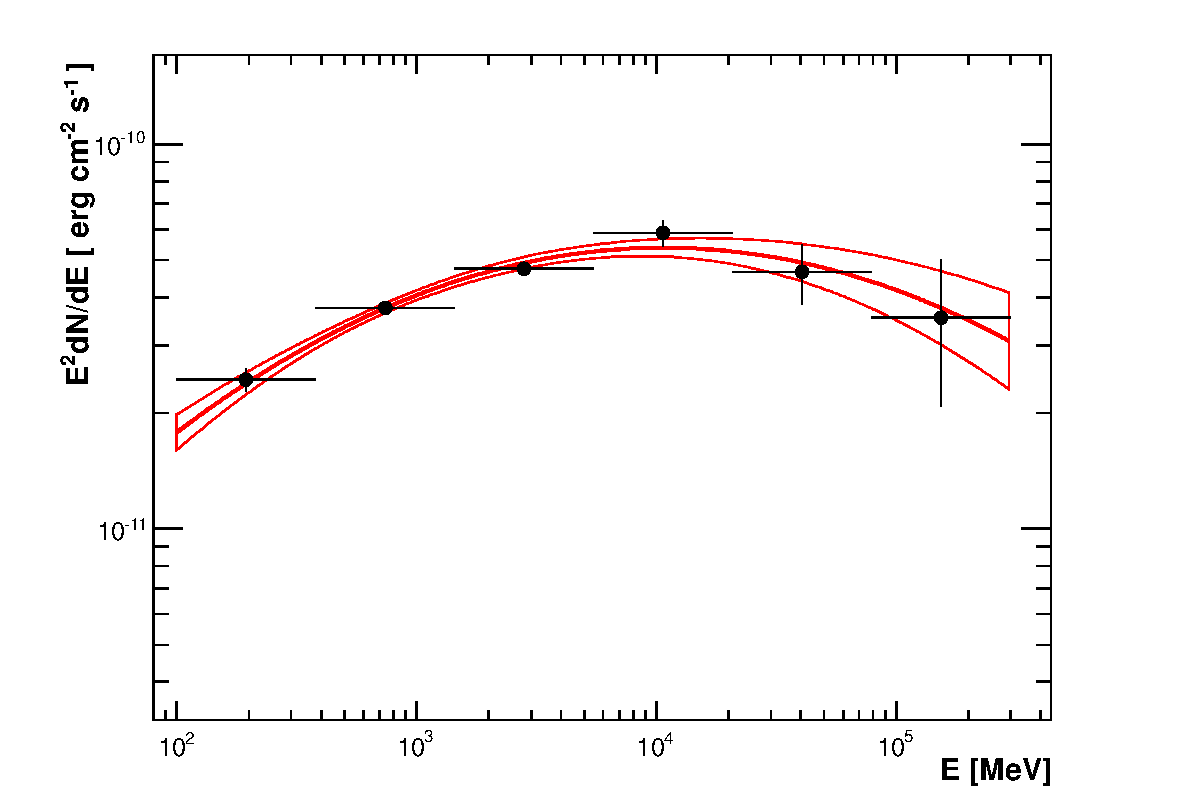
\includegraphics[width=\textwidth]{icrc2013_89_01}
%  \caption{Schematic view of the package. The grey boxes are the command-line tools ran by the user during the data analysis.}
%  \label{fig:idea}
% \end{figure*}


%A schematic view of the package and the idea behind is given in Fig.~\ref{fig:idea}. 
The main features of this package can be summarised as follows:

\begin{itemize}
\item It uses the ST to analyse the LAT data ({\tt FITS} file production,
minimisation, etc...). The {\tt Enrico} command line tools are just front-ends
for functions and classes in the {\tt Enrico} Python package.
\item Analysis is simplified, {\tt Enrico} generates {\tt Xml} model files, {\tt FITS} files and paper-quality plots with a few commands.
\item Results are reproducible, because configuration files and logs are used.
\item Good default options that are suitable for most analyses.
\item Control plots were added to ensure the reliability of the analysis.
\end{itemize}

Written in Python, the code is portable and does not rely on the CPU architecture nor on the ST version. Documentation, tutorial and instructions for installation are available at \url{http://enrico.readthedocs.org}. 

The {\tt Enrico} package includes a job submission module allowing some parallelisation of the tasks, mainly for spectra (energy bins) and light curves (time bins). Currently the MPIK\footnote{\url{http://www.mpi-hd.mpg.de/}} and LAPP\footnote{\url{http://lapp.in2p3.fr/}} clusters are supported but others can easily be added by the user.

\section{A simple analysis}

\subsection{Prepare and run your analysis}

Few steps need to be done before actually running the \Fermi analysis. The command-line tools work with a configuration file that needs to be generated. This is done by:
\mbox{{\tt> enrico\_config PKS2155.conf}} 
where {\tt PKS2155.conf} is the name of the configuration files that will be created. For this exemple, the blazar PKS~2155-304 has been analysed using data from MET=239557418 to MET=271093418 with an energy range from 100~MeV to 300~GeV.

Few questions will be asked about the analysis to perform (source name, position, time, energy range, etc...). The \Fermi data analysis uses a sky model written in an xml file. The package reads the 2FGL catalogue \cite{2012ApJS..199...31N} to generate a coresponding xml model using the tool :

\mbox{{\tt> enrico\_xml PKS2155.conf}}

The produced xml file contains all the sources with the user-defined region of interest plus 10 degrees. Only sources within 3 degrees around the source have their parameters free to vary. Several spectral models are supported (PowerLaw, PowerLaw2, LogParabola, PLExpCutoff, Generic). At this point, the likelihood analysis implemented in {\tt gtlike}, can be simply performed with the command :

\mbox{{\tt enrico\_sed PKS2155.conf}}

A full spectrum and also data points (see Fig.~\ref{fig:SED}) are then computed. The covariance matrix obtained during the minimisation process is then used to compute the 68\% error contour also called butterfly. If the source is not detected (i.e. below the user-defined TS), an upper limit is computed.

Lightcurves (Fig.~\ref{fig:LC}) and TS maps can be produced by {\tt Enrico} using :

\mbox{{\tt> enrico\_lc PKS2155.conf}}

\mbox{{\tt> enrico\_tsmap PKS2155.conf}}

The previous commands run several jobs either in parallel by submitting them to a cluster or sequentially one after the other. A single job is very similar to a spectrum calculation. {\tt FITS} files that are need by {\tt gtlike} are produced and the minimisation is performed either in time bins (light-curves) or in space bins (TS map). For each tool, the generation of the {\tt FITS} files can be skipped if they have already been produced in a previsous analysis. This allows to save CPU time in the cases of recomputation of the best-fit values after a change in the sky model for exemple.

 \begin{figure}[ht!]
  \centering
  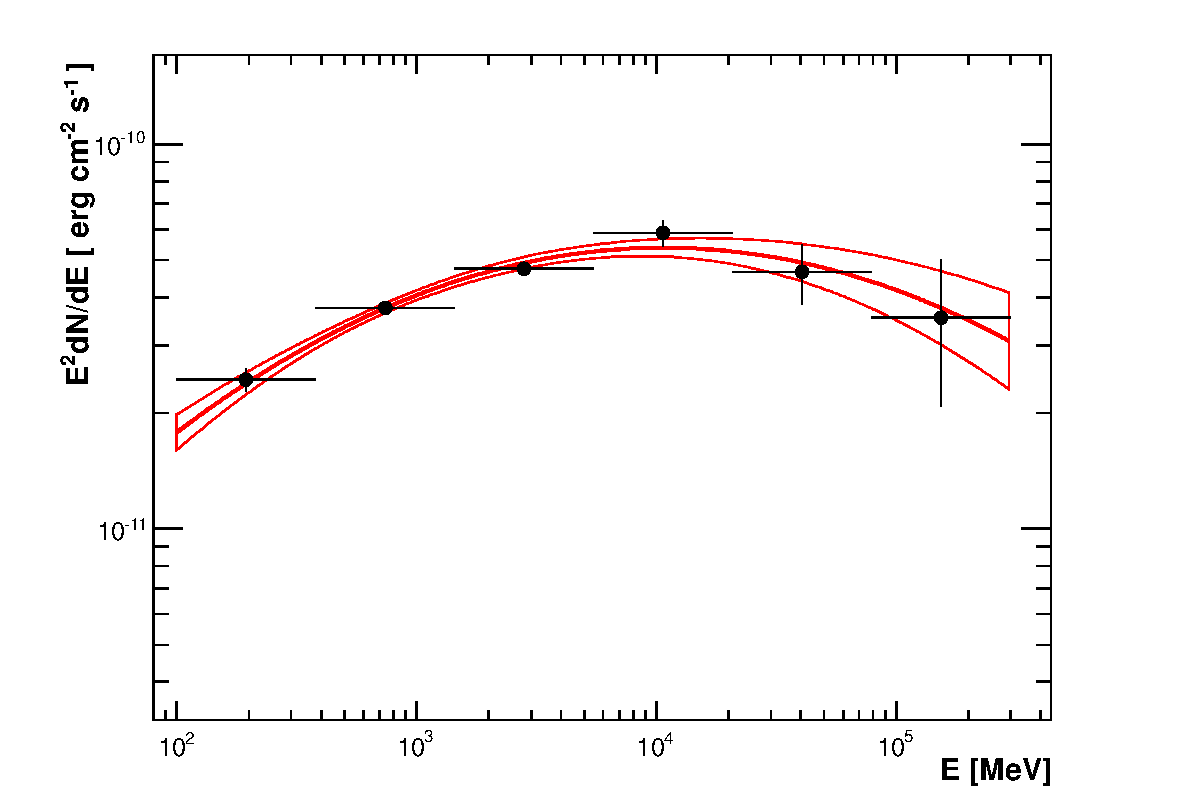
\includegraphics[width=0.49\textwidth]{icrc2013_89_01}
  \caption{Spectral energy distribution of the Blazar PKS 2155-304 as obtained with {\tt Enrico} and the tools {\tt enrico\_sed} and {\tt enrico\_plot\_sed}.}
  \label{fig:SED}
 \end{figure}

 \begin{figure}[ht!]
  \centering
  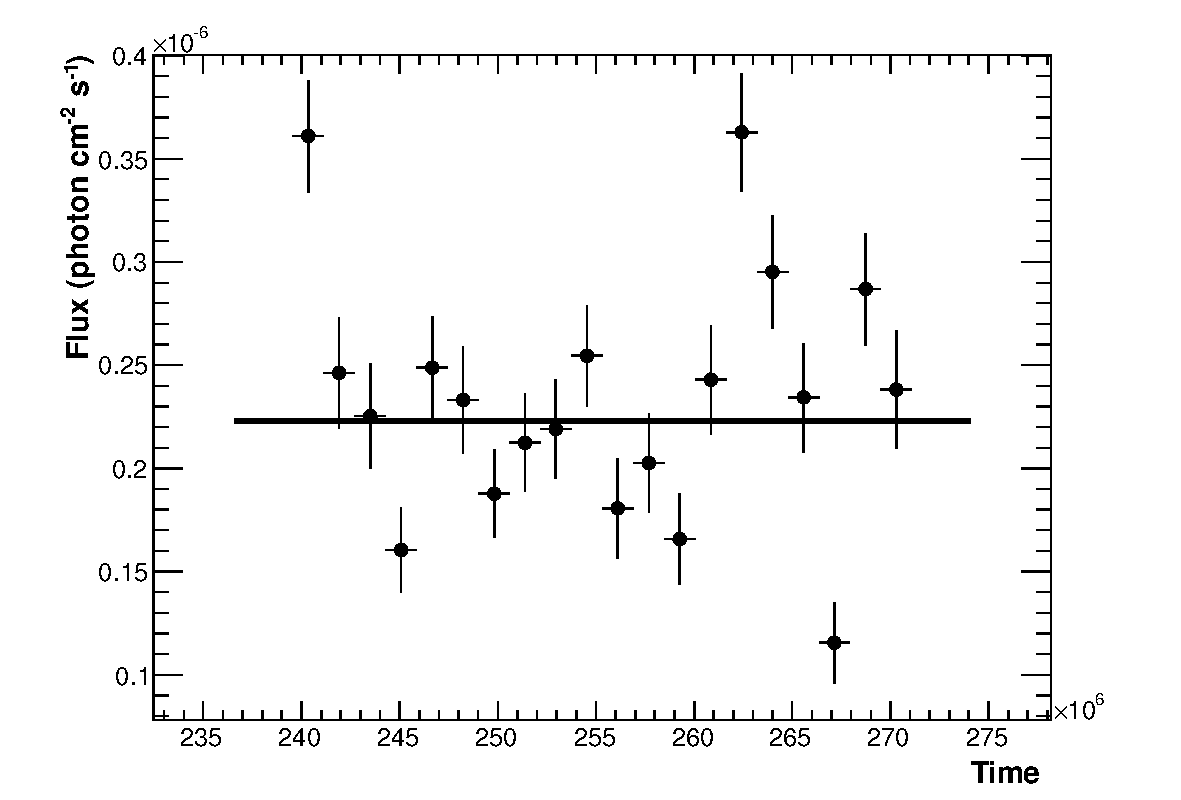
\includegraphics[width=0.49\textwidth]{icrc2013_89_02}
  \caption{light-curve of the Blazar PKS 2155-304 as obtained with {\tt Enrico} and the tools {\tt enrico\_lc} and {\tt enrico\_plot\_lc}.}
  \label{fig:LC}
 \end{figure}

{\tt Enrico} has a module to produce paper-quality plots, saved in {\tt eps}, {\tt .C} (ROOT format) and {\tt png}:

\mbox{{\tt> enrico\_plot\_sed PKS2155.conf}}

\mbox{{\tt> enrico\_plot\_lc PKS2155.conf}}

\mbox{{\tt> enrico\_plot\_tsmap PKS2155.conf}}


It is also posible to compute the log-likelihood value of several spectral models assumed for the source of interest. Tested models are PowerLaw, LogParabola and PLExpCutoff. The tool is called by :

\mbox{{\tt> enrico\_testmodel PKS2155.conf}}


\subsection{Configuration file}
The configuration file is a {\tt ascii} file automaticaly generated by the package but that can be edited by the user. An exemple is presented in Fig.~\ref{fig:conf}.

 \begin{figure}[t]
  \centering
  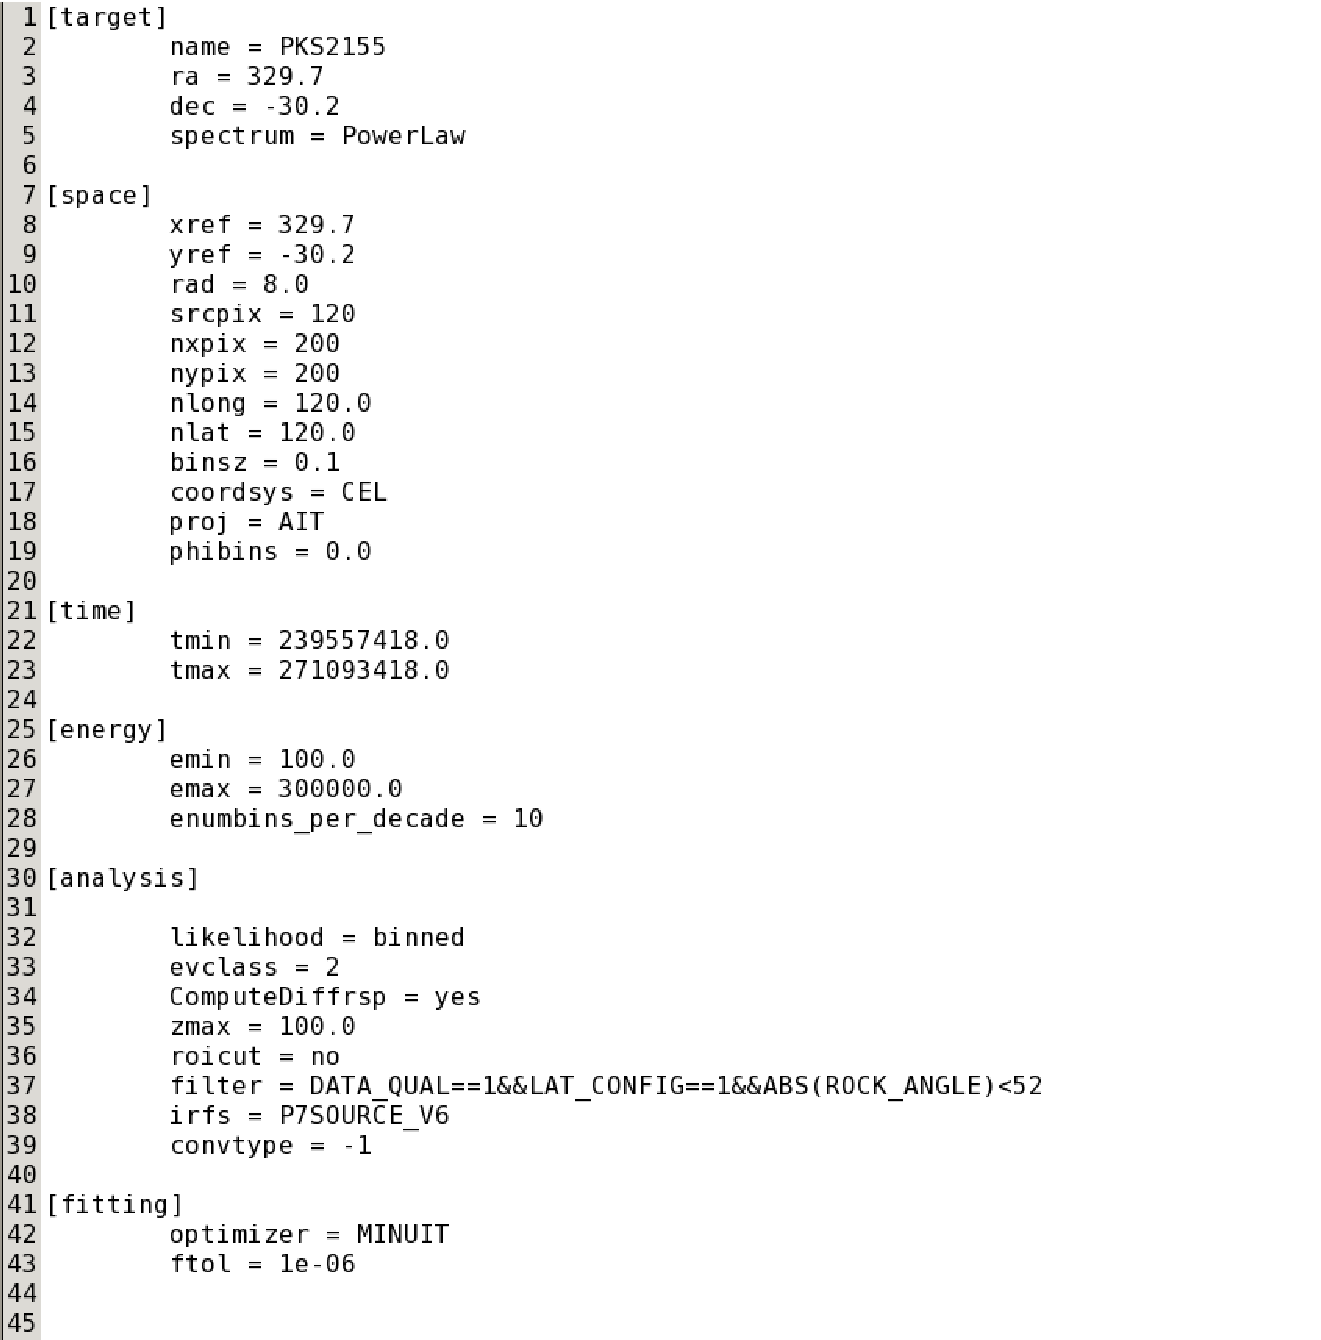
\includegraphics[width=0.4\textwidth]{icrc2013_89_03}
  \caption{Exemple of a configuration file for {\tt Enrico}.}
  \label{fig:conf}
 \end{figure}

A configuration file is divided in sections. It contains simple sections (e.g. \textbf{energy}, \textbf{time}) in which the user defines cuts applied for all analysis. More specific sections exist and are used by only one tool (e.g. section \textbf{spectrum} for {\tt enrico\_sed}).


\subsection{Check your results}

While in principle straightforward, the ST might be tricky to use and the results of a \Fermi data analysis should be checked. {\tt Enrico} proposes few control plots in order to ensure the reliability of an analysis. 

For the spectrum, a count plot (Fig.~\ref{fig:control1}) and a residual plot are produced. For the light-curves, a plot, $N_{\rm pred}/\sqrt{N_{\rm pred}}$ vs Flux$/\Delta$ Flux (Fig.~\ref{fig:control2}), is made to unsure the good computation of the errors since the two values must be correlated. Count map, model map and residual map (Fig.~\ref{fig:Map}) are also automaticaly produced and can be used to see if a source should be added to the sky model or have its paramters free.


 \begin{figure}[t]
  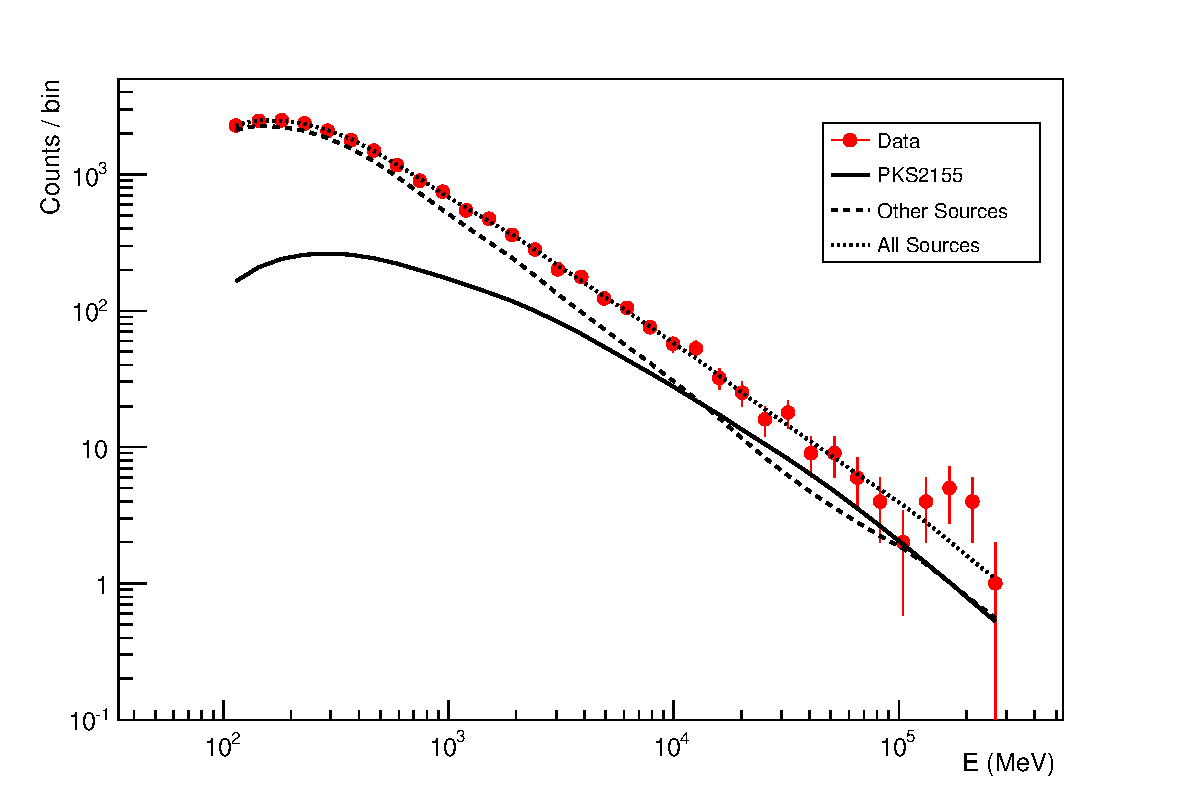
\includegraphics[width=0.49\textwidth]{icrc2013_89_04}
  \caption{{\tt Counts plot} showing the number of count per bins and the different model components (Source, other objects and total) as fitted by {\tt gtlike}.}
\label{fig:control1}
 \end{figure}

 \begin{figure}[t]
  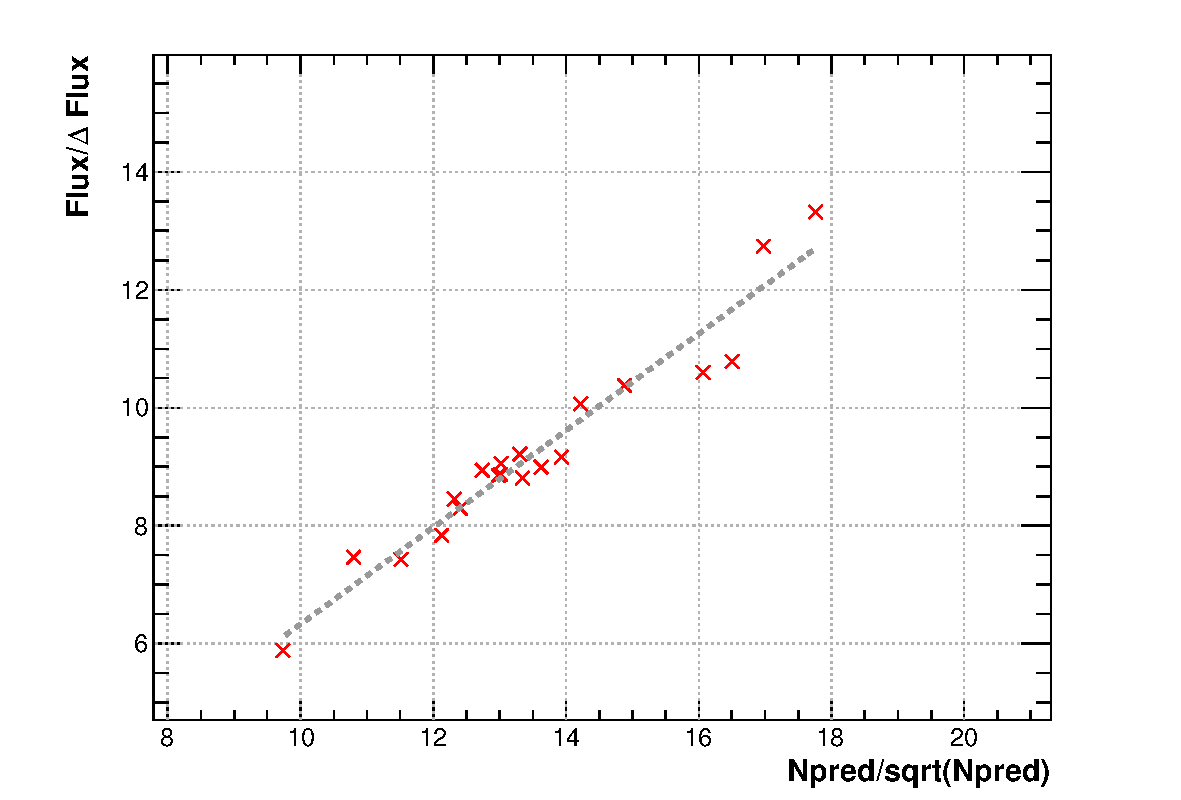
\includegraphics[width=0.49\textwidth]{icrc2013_89_05}
  \caption{Plot ($N_{\rm pred}/\sqrt{N_{\rm pred}}$ vs Flux$/\Delta$ Flux) used to decide whether the errors in the light-curves are well computed.}
\label{fig:control2}
 \end{figure}

\section{Conclusions}

{\tt Enrico} is a powerful tool written in {\tt Python} to run the \Fermi ScienceTools. With the addition of debug plots and submission of several job on cluster of CPUs, rapid, robust and reproducible analyses can be performed easily.
The implementation of automatic download of data from the FSSC data server for a given sky region, energy band and time range is being
implemented as part of the {\tt astroquery.fermi} module (see \url{https://github.com/astropy/astroquery}), which is a Python package
to access public astronomy data services on the web.

We invite the reader to try {\tt Enrico} for \Fermi LAT data analysis.
Start by downloading it from \url{https://github.com/gammapy/enrico}
and browsing the documentation at \url{http://enrico.readthedocs.org}.

 \begin{figure}[t]
  \centering
  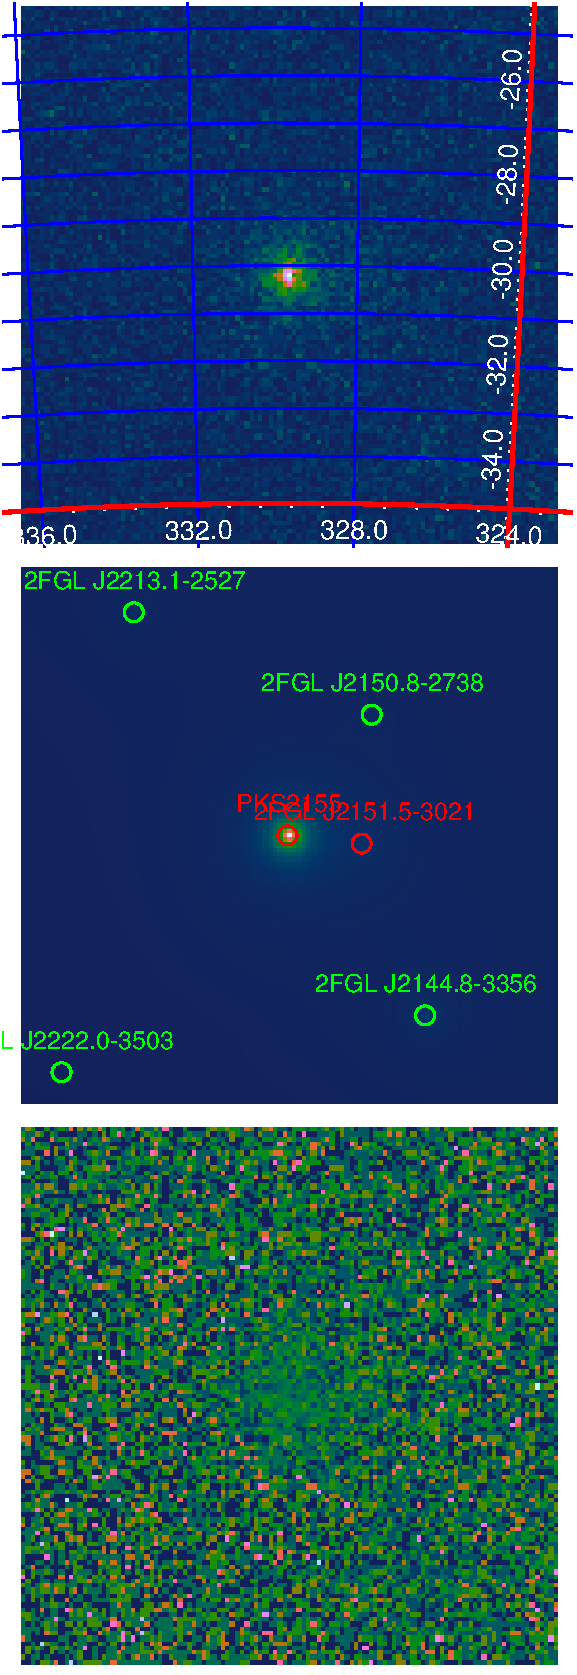
\includegraphics[width=0.4\textwidth]{icrc2013_89_06}
  \caption{From top to bottom: Counts map, Model map and residuals. The first two maps are produced with the ST (with {\tt gtbin} and {\tt gtmodelmap}) and the last is produced by {\tt Enrico} to allow the user to check the sky model.}
  \label{fig:Map}
 \end{figure}


\begin{thebibliography}{}


\bibitem{2012ApJS..199...31N} Nolan, P.~L., Abdo, A.~A., Ackermann, M., et al.\ 2012, ApJS, 199, 31 

\end{thebibliography}

\end{document}
